
\section{Sources Detected by \Actitle{LAT}}
\seclabel{sources_detected_fermi} 

\begin{figure}[htbp]
  \centering
    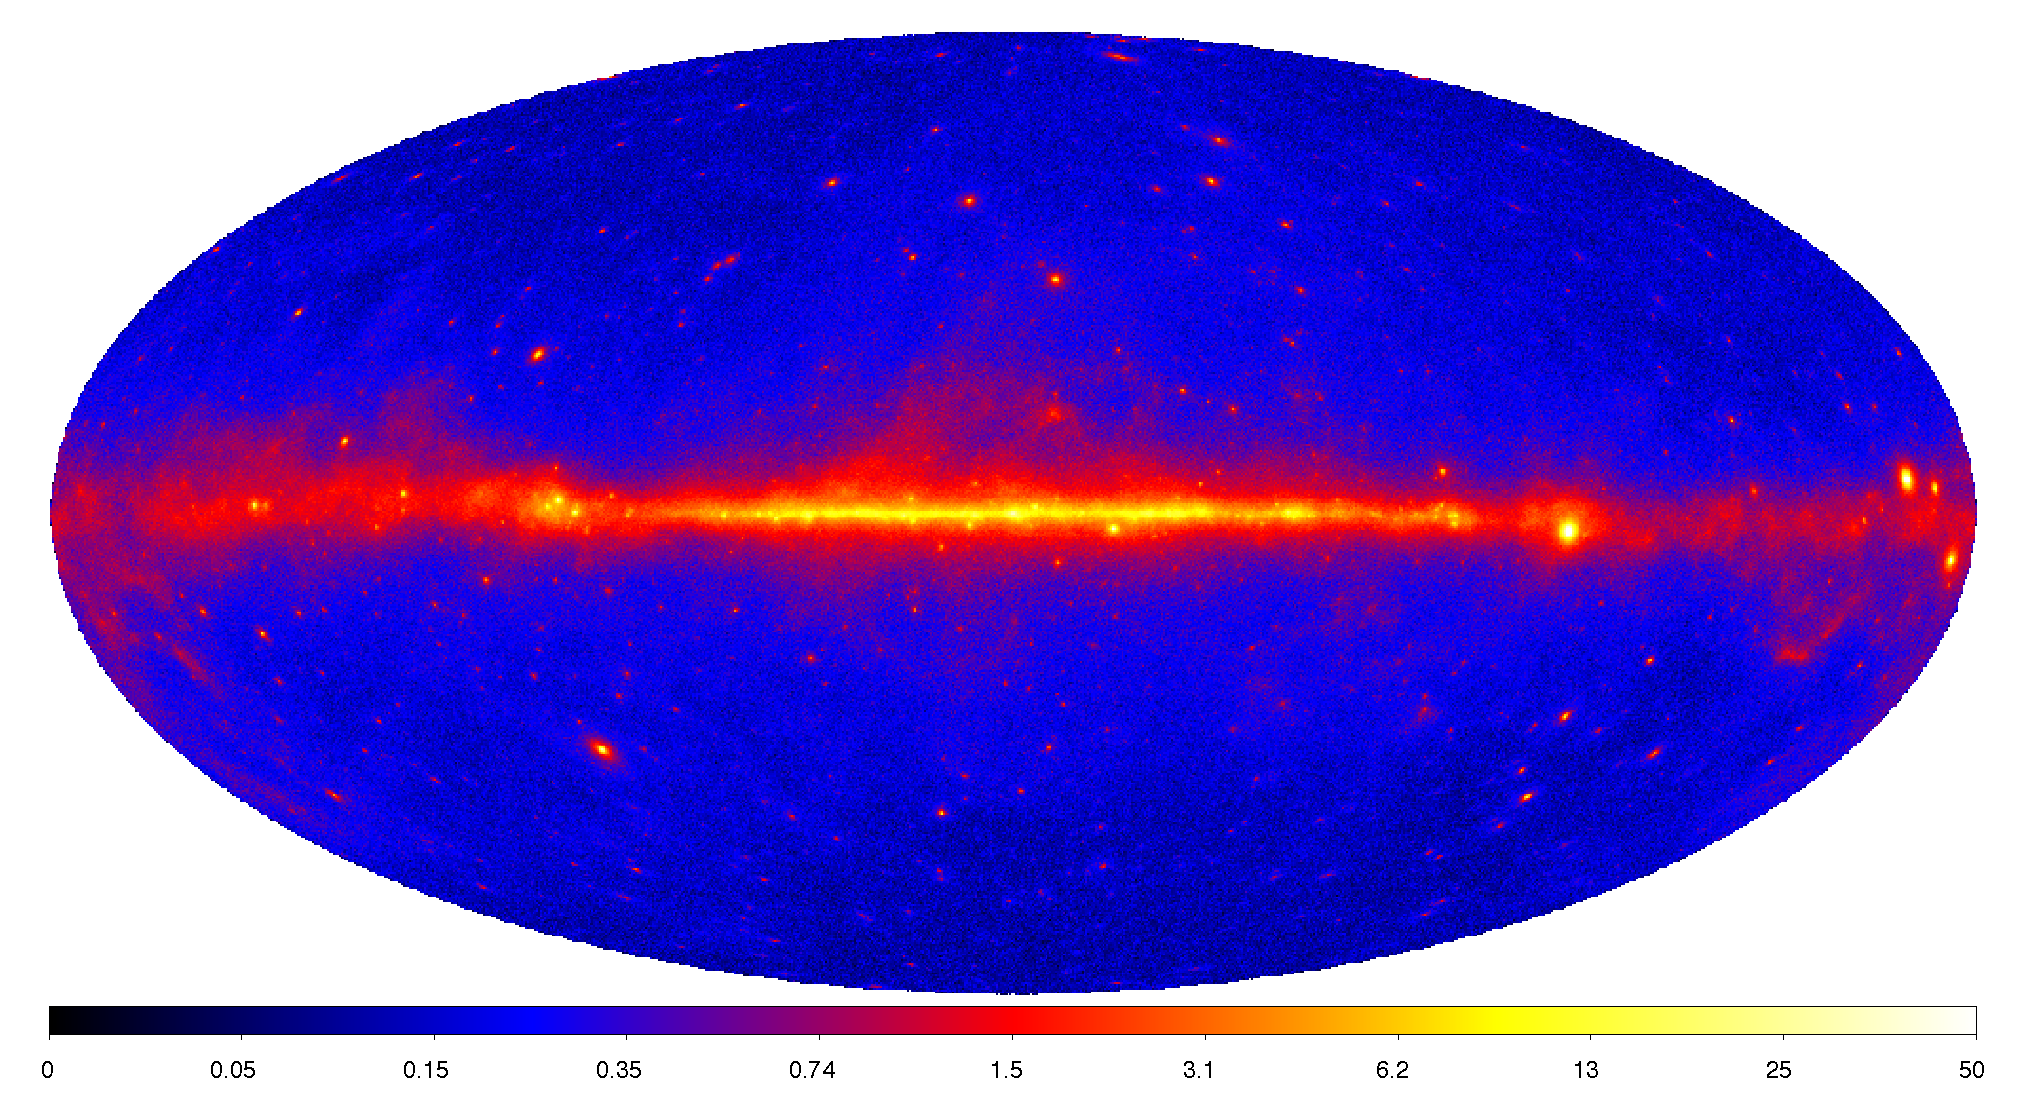
\includegraphics[width=\textwidth]{chapters/introduction/figures/lat_skymap_2fgl.pdf}
  \caption{
  An Aitoff projection map of the $\gamma$-ray sky observed by the
  \ac{LAT} with a 2 years exposure.  This map is integrated in the
  energy range from $100\unitspace\mev$ to $10\unitspace\gev$ in units
  of $10^{-7}\erg\unitspace\cm^{-2}\second^{-1}\steradian^{-1}$.  This figure is
  from \cite{nolan_2012_fermi-large}.
  }
  \figlabel{lat_skymap_2fgl}
\end{figure}

\figref{lat_skymap_2fgl} shows a map of the $\gamma$-ray sky observed
with two years of data. From this map, one can clearly observed a
strongly-structured anisotropic component of the $\gamma$-ray emission
from the galaxy. In addition, many individual sources of $\gamma$-rays
can be viewed. In \subsecref{galactic_diffuse_and_isotropic}, we
discuss the Galactic diffuse and isotropic $\gamma$-ray background. In
\subsecref{2fgl}, we discuss \ac{2FGL}, a catalog of point-like
sources detected by the \ac{LAT}. In \subsecref{2pc}, we discuss
\ac{2PC}, a catalog of pulsars detected by the \ac{LAT}.  Finally,
in \subsecref{pwn_detected_lat} we discuss \acp{PWN} detected by the
\ac{LAT}.


\subsection{The Galactic Diffuse and Isotropic Gamma-ray Background}
\subseclabel{galactic_diffuse_and_isotropic}

the interaction of cosmic-ray electrons and protons with the gas in our
Milky Way (through the \pion and bremsstrahlung process) and with the
Galactic radiation fiels (through the \ac{IC} process).

Much work has gone into theoretically modeling the diffuse
$\gamma$-ray emission. The most advanced theoretical model
of Galactic emission from or galaxy comes from the \galprop code
\citep{strong_1998a_propagation-cosmic-ray,moskalenko_2000a_anisotropic-inverse}.
In addition, significant work by \cite{abdo_2009a_fermi-large} and
\cite{ackermann_2012a_fermi-lat-observations} have gone into comparing
these theoretical predictions to the observed $\gamma$-ray intensity
distribution observed by the \ac{LAT}.

In addition to an anisotropic Galactic diffuse background, the \ac{LAT}
observes an isotropic component to the $\gamma$-ray distribution.
This emission is believed to be a composite of unresolved extragalactic
point-like sources as well as a residual charged-particle background.
\cite{abdo_2010a_spectrum-isotropic} presents detailed measurements of
isotropic background observed by the \ac{LAT}.

The \galprop predictions for the $\gamma$-ray background are not
accurate enough for the analysis of point-like (and $\sim1\degree$
large extended sources).  Therefore, an improved data-driven model
of the Galactic diffuse background has been devised where components
of the \galprop model are fit to the observed $\gamma$-ray emission.
This data-driven model is described in \cite{nolan_2012_fermi-large}.


\subsection{\Actitle{2FGL}}
\subseclabel{2fgl}

Using 2 years of observations, the \ac{LAT} collaboration produces
a list of 1873 $\gamma$-ray-emitting sources detected significantly
in the $100\unitspace\mev$ to $100\unitspace\gev$ energy range
\cite{nolan_2012_fermi-large}.  Using the maximum-likelihood analysis
method described in \chapref{maximum_likelihood_analysis}, \ac{2FGL}
computed for each source the position and uncertainty on this error. In
addition, the catalog produced the best-fit spectral parameters assuming
this source has a power-law spectrum or a log-normal spectrum.
Primarily, the catalog assumed sources to be point like. But twelve
previously-published sources were included as being spatially extended
with the spatial model taken from the prior publications.

Of these 1873 sources, 127 were firmly identified with a multiwavelength
counterpart.  A source is only firmly identified if it meets one of three
criteria. First, it would have periodic variability.  This applies to
pulsars and high-mass binaries.  Second, it could have a matching spatial
morphology. This primarily applies to \acp{SNR} and \acp{PWN}. Finally,
it could have correlated variability. This applies primarily to \ac{AGN}.
In total, \ac{2FGL} clearly identifies 83 pulsars, 28 \acp{AGN}, 6
\acp{SNR}, 4 \acp{HMB}, 3 \acp{PWN}, 2 normal galaxies, and one nova
\cite{nolan_2012_fermi-large}.

In addition, 1171 sources are included in the looser criteria that
they are potentially associated with a multiwavelength counterpart.
Using these looser criteria, 86 sources are associated with pulsars, 25
with \acp{PWN},  98 with \acp{SNR}.  Finally, 162 were flagged as being
potentially spurious due to residuals included by incorrectly modeling
the galactic diffuse emission.

\subsection{\Actitle{2PC}}
\subseclabel{2pc}

Using 3 years of data, the \ac{LAT} collaboration produced a
list of 117 pulsars significantly detected by the \ac{LAT} called
\acf{2PC} \citep{abdo_2013a_second-fermi}.  To search for pulsars with
\ac{LAT}-detected pulsations, commonly pulsars are first detected at
either radio or x-ray energies. Then, a multiwavelength model of the
pulsar's rotational period is used to fold the $\gamma$-ray photons
coming from the direction of the pulsar.  The H-test is used to compute
the significance of pulsations \citep{de-jager_1989a_poweful-periodic}
and typically a $5\sigma$ threshold is used for claiming a significant
detection.  This method was used to discover 61 of the $\gamma$-ray
emitting pulsars.

In addition, some pulsars are known to emit only $\gamma$-rays.
These sources search for by blindly searching in the $\gamma$-ray data
for periodic emission. This method was used to detect 36 pulsars.

Finally, in the third method, the positions of unidentified \ac{LAT}
sources which could potentially be associated with pulsars are search in
radio to look for pulsar emission. This method has lead to the detection
of 20 new \acp{MSP}.

In total \ac{2PC} contains a list of 42 radio-loud pulsars, 35 radio-quiet
pulsars, and 40 $\gamma$-ray \acp{MSP}.

\subsection{\Acptitle{PWN} Detected by \Actitle{LAT}}
\subseclabel{pwn_detected_lat}

In addition to detecting over 100 pulsars, the \ac{LAT} has detected
several \acp{PWN}.  In situations where the \acp{PWN} has an associated
\ac{LAT}-detected pulsar, most commonly the spectral analysis of the
\ac{PWN} is performed only during times in the pulsar phase where the
pulsar emission is at a minimum. For some pulsars, such as \hessj{1825},
there is no associated \ac{LAT}-detected pulsar and the spectral analysis
can be performed without cutting on pulsar phase.

\subsubsection{Crab}

\begin{figure}[htbp]
  \centering
    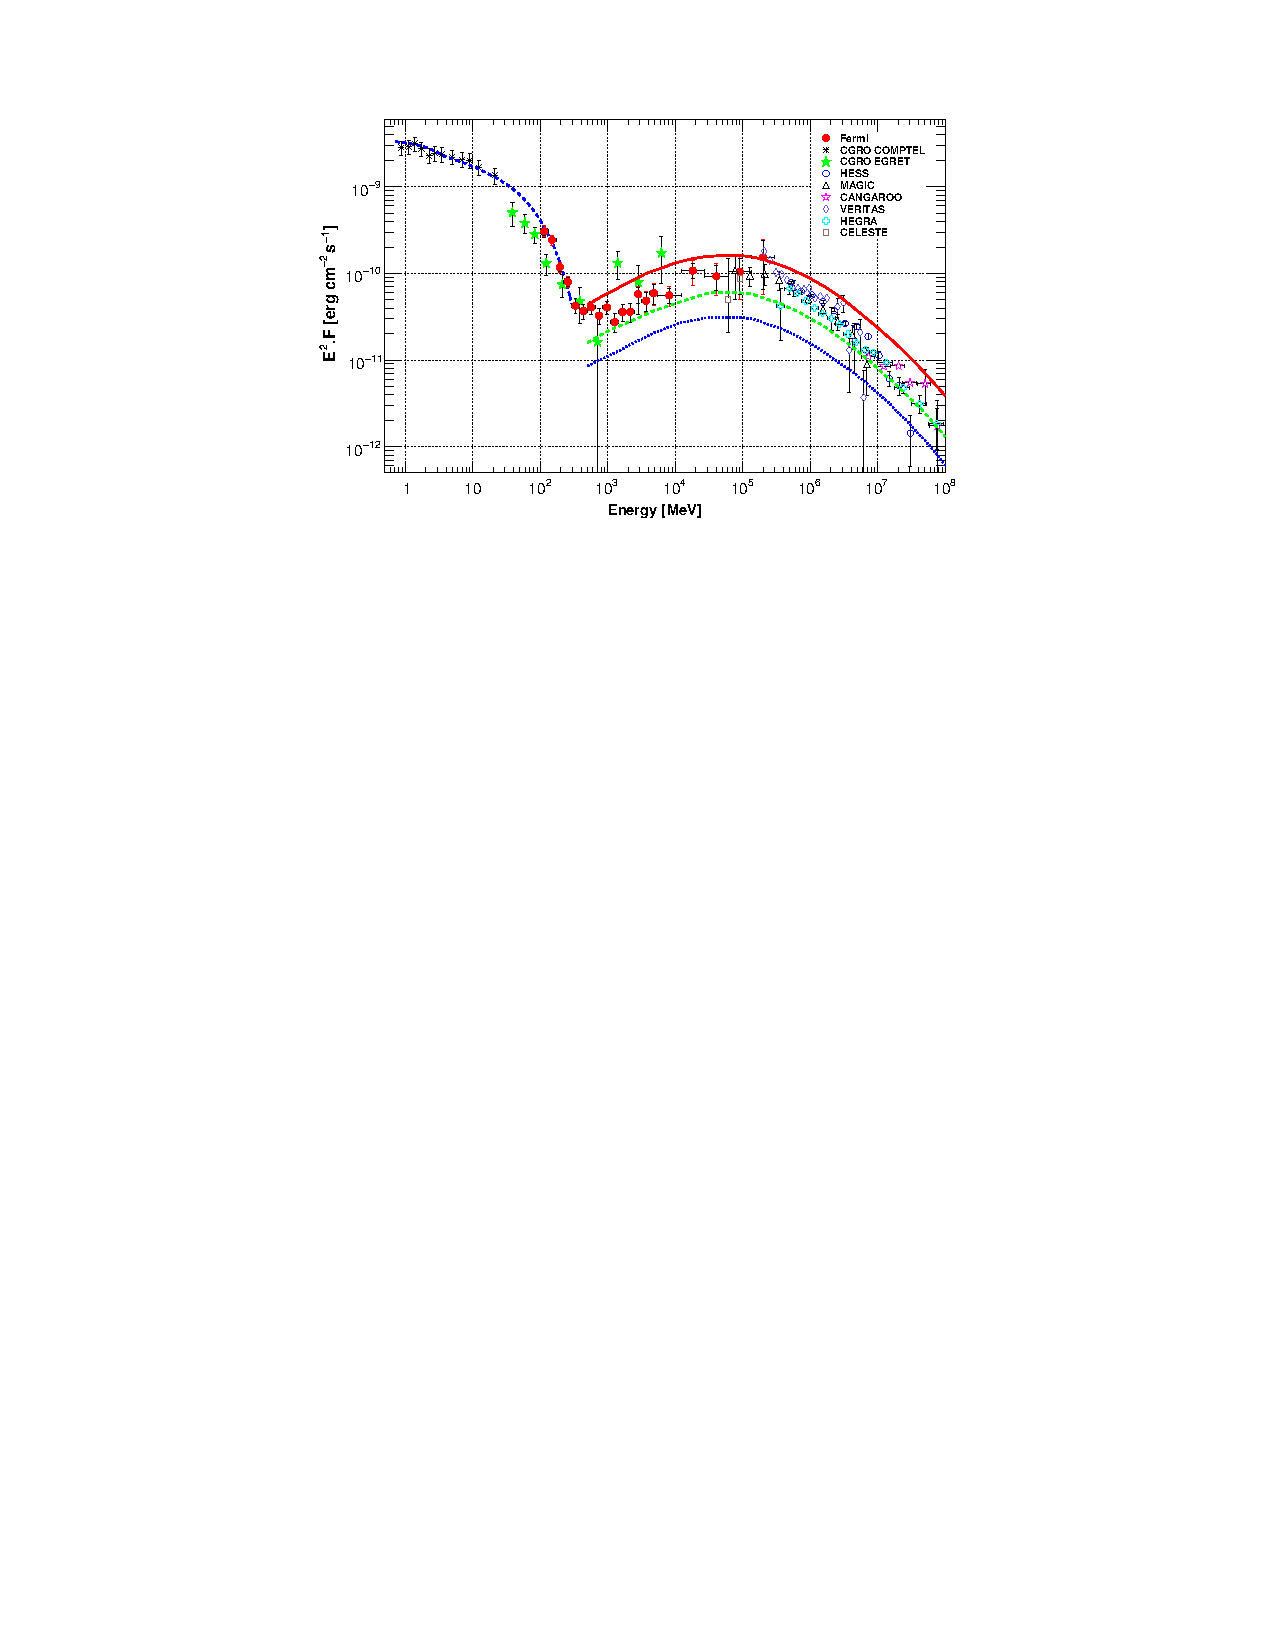
\includegraphics{chapters/introduction/figures/crab_spectrum.pdf}
  \caption{
    The \ac{SED} of the Crab nebula observed by the \ac{LAT} as
    well as a variety of other instruments.
    This figure is from \cite{abdo_2010a_fermi-large}.
  }
  \figlabel{crab_spectrum}
\end{figure}

The Crab nebula, introduced in \subsecref{pwn}, was first detected
in $\gamma$-rays by \ac{EGRET}.  Observations of the Crab by the
\ac{LAT} provide unprecedented resolution on the $\gamma$-ray emission
\cite{abdo_2010a_fermi-large}.  The Crab nebula shows a very strong
spectral break in the \ac{LAT} energy band, and the $\gamma$-ray emission
is interpreted as being the combination of a synchrotron component at low
energy and an \ac{IC} component at high energy.

In addition, $\gamma$-ray emission from the Crab nebula has
been observed to be variability in time and have flaring periods
\citep{abdo_2011a_gamma-ray-flares}.  The Crab was observed to have
an extreme flare in 2011 \citep{buehler_2012a_gamma-ray-activity}.
This variability is challenging to understand given conventional models
of \ac{PWN} emission.

\subsubsection{\velax}

\begin{figure}[htbp]
  \centering
    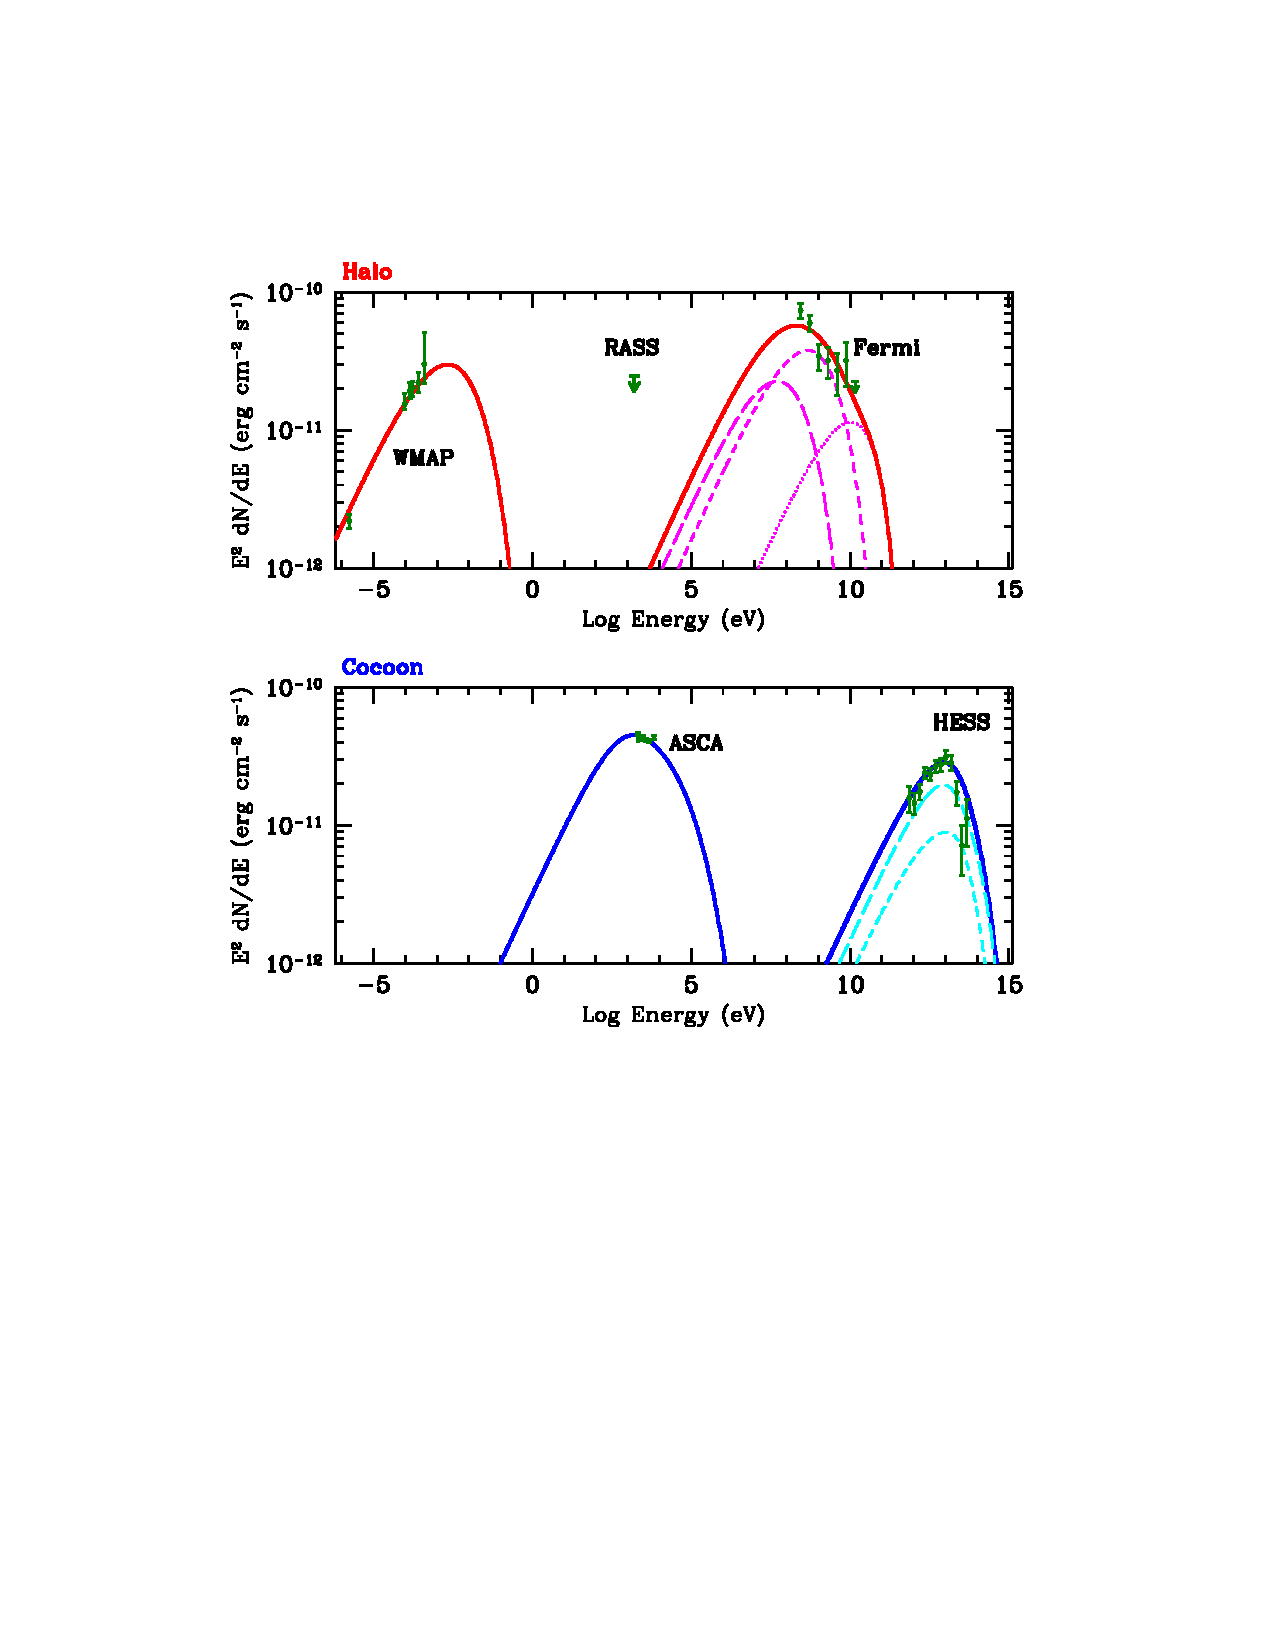
\includegraphics{chapters/introduction/figures/vela_x_sed_two_populations.pdf}
    \caption{The \ac{SED} of \velax observed at radio, x-ray,
      $\gamma$-ray, and \ac{VHE} energies. The emission was suggested
      by \citep{abdo_2010c_fermi-large} to be driven by two pollutions
      of electrons.  In this model, the lower-energy electron population
      powers the radio and $\gamma$-ray emission adn the higher-energy
      electron population powers the x-ray and \ac{VHE} emission.
      This figure is from \cite{abdo_2010c_fermi-large}.}
  \figlabel{vela_x_sed_two_populations}
\end{figure}


The \velax is the \ac{PWN} powered by the Vela pulsar.  It was first
observed by \cite{rishbeth_1958a_radio-emission}, at \ac{VHE} energies
by \cite{aharonian_2006a_first-detection}, and then at \gev energies
by \ac{AGILE} in \cite{pellizzoni_2010a_detection-gamma-ray}.
The detailed multiwavelength spectra of \velax is plotted in
\figref{vela_x_sed_two_populations}.  Based upon the morphological and
spectral disconnect, \citep{abdo_2010c_fermi-large} argued that emission
was not consistent with a single population of electrons powering the
multiwavelength emission. They suggested instead that the emission could
come from from two populations of electrons.

\subsubsection{\mshfifteenfiftytwo}

The \ac{SNR} \snrg{320.4} (\mshfifteenfiftytwo)
\cite{caswell_1981a_high-resolution-radio} is commonly
associated with PSR\,B1509$-$58 \cite{seward_1982a_x-ray-pulsar}.
\cite{seward_1982a_x-ray-pulsar} observed a diffuse nebula surrounding the
pulsar. This was interpreted by \cite{trussoni_1996a_rosat-observations}.
This \ac{PWN} was discovered at \ac{VHE} energies by
\cite{aharonian_2005a_discovery-extended} and subsequently at \gev
energies by \cite{abdo_2010a_detection-energetic}

\subsubsection{\hessj{1825}}

\hessj{1825} is an extended ($\sim0\fdg5$) \ac{VHE} sources
first detected during the \ac{HESS} survey of the inner
galaxy \citep{aharonian_2006a_h.e.s.s.-survey}.  It was
interpreted by \cite{aharonian_2005a_possible-association}
as being a \ac{PWN} powered by \psrj{1826} \citep[also known as
\psrb{1823},][]{clifton_1992a_high-frequency-survey}.  Surrounding the
pulsar is a diffuse $\sim 5'$ nebula \cite{finley_1996a_morphology-young}.
The large $R_\gamma/R_X$ ratio can be understood in terms of the
different for the synchrotron-emitting and \ac{IC}-emitting electrons
\citep{aharonian_2006a_h.e.s.s.-survey}.

This source was subsequently detected by
\cite{grondin_2011a_detection-pulsar} at \gev energies.  Interestingly,
the \ac{VHE} emission from \hessj{1825} was observed to have an
energy-dependent morphology, with the size decreasing with increasing
energy \citep{aharonian_2006a_energy-dependent}.  This can e explained
under the assumption of \ac{IC} emission caused by electrons from a
pulsar whose spin-down energy is constantly decreasing.

\subsubsection{\hessj{1640}}

The \ac{VHE} source \hessj{1640} was discovered by
\ac{HESS} \citep{aharonian_2006a_h.e.s.s.-survey}.  This
\ac{VHE} source is spatially-coincident with \snrg{338.3}
\citep{shaver_1970a_galactic-radio}.  X-ray observations by
\xmmnewton uncovered a spatially coincident X-ray nebula and within it
a point-like source \cite{funk_2007a_xmm-newton-observations}.
This point-like source is believed to be a neutron star powering the
nebula, but pulsations have not been detected from it.
\cite{slane_2010_fermi-detection} discovered an associated \gev source.
These observations have been interpreted in terms of a pulsar/\ac{PWN}
hypothesis.

\subsubsection{\hessj{1857}}

\hessj{1857} was also discovered by \ac{HESS}
\cite{aharonian_2008a_very-high-energy-gamma-ray}
It was suggested that \hessj{1857} is a \ac{PWN} powered by
\psrj{1856} \cite{hessels_2008a_j18560245:-arecibo}.
\hessj{1857} was also detected by the \ac{LAT}

\subsubsection{\hessj{1023}}

\ac{HESS} discovered \hessj{1023} in the region of the young stellar
cluster Westerlund 2 \cite{aharonian_2007a_detection-extended}.  This same
source was subsequently detected by the \ac{LAT} in the off-peak region
surrounding \psrj{1023} \citep{ackermann_2011a_fermi-lat-search}.
\cite{h.e.s.s.collaboration_2011a_revisiting-westerlund} proposed that
the emission could either be due to an \acp{PWN} or due to hadronic
interactions of cosmic rays accelerated in the open stellar cluster
interacting with molecular clouds.

We will discuss the population of $\gamma$-ray emitting \acp{PWN}
in \chapref{population_study}.
